\documentclass[12pt]{article}

%%%%%%%%%%%%%%%%%%%%%%%%%%%%%%%%%%%%%%%%%%%%%%%%%%%%%%%%%%%%%%%%%%%%%%%%%%%%%%%%
%                           Package preset for homework
%%%%%%%%%%%%%%%%%%%%%%%%%%%%%%%%%%%%%%%%%%%%%%%%%%%%%%%%%%%%%%%%%%%%%%%%%%%%%%%%
% Miscellaneous
\usepackage[margin=1in]{geometry}
\usepackage[utf8]{inputenc}
\usepackage{indentfirst}
\usepackage{blindtext}
\usepackage{graphicx}
\usepackage{xr-hyper}
\usepackage{hyperref}
\usepackage{enumitem}
\usepackage{color}
\usepackage{float}
% Math
\usepackage{latexsym}
\usepackage{amsfonts}
\usepackage{amssymb}
\usepackage{amsmath}
\usepackage{commath}
\usepackage{amsthm}
\usepackage{bbold}
\usepackage{bm}
% Physics
\usepackage{physics}
\usepackage{siunitx}
% Code typesetting
\usepackage{listings}
% Citation
\usepackage[authoryear]{natbib}
\usepackage{appendix}
\usepackage[capitalize]{cleveref}
% Title & name
\title{Homework}
\author{Tien Vo}
\date{\today}


%%%%%%%%%%%%%%%%%%%%%%%%%%%%%%%%%%%%%%%%%%%%%%%%%%%%%%%%%%%%%%%%%%%%%%%%%%%%%%%%
%                   User-defined commands and environments
%%%%%%%%%%%%%%%%%%%%%%%%%%%%%%%%%%%%%%%%%%%%%%%%%%%%%%%%%%%%%%%%%%%%%%%%%%%%%%%%
%%% Misc
\sisetup{load-configurations=abbreviations}
\newcommand{\due}[1]{\date{Due: #1}}
\newcommand{\hint}{\textit{Hint}}
\let\oldt\t
\renewcommand{\t}[1]{\text{#1}}

%%% Bold sets & abbrv
\newcommand{\N}{\mathbb{N}}
\newcommand{\Z}{\mathbb{Z}}
\newcommand{\R}{\mathbb{R}}
\newcommand{\Q}{\mathbb{Q}}
\let\oldP\P
\renewcommand{\P}{\mathbb{P}}
\newcommand{\LL}{\mathcal{L}}
\newcommand{\FF}{\mathcal{F}}
\newcommand{\HH}{\mathcal{H}}
\newcommand{\NN}{\mathcal{N}}
\newcommand{\ZZ}{\mathcal{Z}}
\newcommand{\RN}[1]{\textup{\uppercase\expandafter{\romannumeral#1}}}
\newcommand{\ua}{\uparrow}
\newcommand{\da}{\downarrow}

%%% Unit vectors
\newcommand{\xhat}{\vb{\hat{x}}}
\newcommand{\yhat}{\vb{\hat{y}}}
\newcommand{\zhat}{\vb{\hat{z}}}
\newcommand{\nhat}{\vb{\hat{n}}}
\newcommand{\rhat}{\vb{\hat{r}}}
\newcommand{\phihat}{\bm{\hat{\phi}}}
\newcommand{\thetahat}{\bm{\hat{\theta}}}

%%% Other math stuff
\providecommand{\units}[1]{\,\ensuremath{\mathrm{#1}}\xspace}
% Set new style for problem
\newtheoremstyle{problemstyle}  % <name>
        {10pt}                   % <space above>
        {10pt}                   % <space below>
        {\normalfont}           % <body font>
        {}                      % <indent amount}
        {\bfseries\itshape}     % <theorem head font>
        {\normalfont\bfseries:} % <punctuation after theorem head>
        {.5em}                  % <space after theorem head>
        {}                      % <theorem head spec (can be left empty, 
                                % meaning `normal')>

% Set problem environment
\theoremstyle{problemstyle}
\newtheorem{problemenv}{Problem}[section]
\newenvironment{problem}[1]{%
  \renewcommand\theproblemenv{#1}%
  \problemenv
}{\endproblemenv}
% Set lemma environment
\newenvironment{lemma}[2][Lemma]{\begin{trivlist}
\item[\hskip \labelsep {\bfseries #1}\hskip \labelsep {\bfseries #2.}]}{\end{trivlist}}
% Set solution environment
\newenvironment{solution}{
    \begin{proof}[Solution]$ $\par\nobreak\ignorespaces
}{\end{proof}}
\numberwithin{equation}{problemenv}

%%% Page format
\setlength{\parindent}{0.5cm}
\setlength{\oddsidemargin}{0in}
\setlength{\textwidth}{6.5in}
\setlength{\textheight}{8.8in}
\setlength{\topmargin}{0in}
\setlength{\headheight}{18pt}

%%% Code environments
\definecolor{dkgreen}{rgb}{0,0.6,0}
\definecolor{gray}{rgb}{0.5,0.5,0.5}
\definecolor{mauve}{rgb}{0.58,0,0.82}
\lstset{frame=tb,
  language=Python,
  aboveskip=3mm,
  belowskip=3mm,
  showstringspaces=false,
  columns=flexible,
  basicstyle={\small\ttfamily},
  numbers=none,
  numberstyle=\tiny\color{gray},
  keywordstyle=\color{blue},
  commentstyle=\color{dkgreen},
  stringstyle=\color{mauve},
  breaklines=true,
  breakatwhitespace=true,
  tabsize=4
}
\lstset{
  language=Mathematica,
  numbers=left,
  numberstyle=\tiny\color{gray},
  numbersep=5pt,
  breaklines=true,
  captionpos={t},
  frame={lines},
  rulecolor=\color{black},
  framerule=0.5pt,
  columns=flexible,
  tabsize=2
}


\title{Homework 1: Phys 5210 (Fall 2021)}


\begin{document}

\maketitle

\begin{problem}{1}

Masses $M$ and $m$ are connected to a system of strings and pulleys as shown.
The strings are massless and inextensible, and the pulleys are massless and
frictionless. The ``floor'' and the ``ceiling'' shown in the figure are fixed
and cannot move. Find the accelerations of $m$ and $M$. The bottom and top
panels are fixed in place and cannot move.

\begin{figure*}[h]
    \centering
    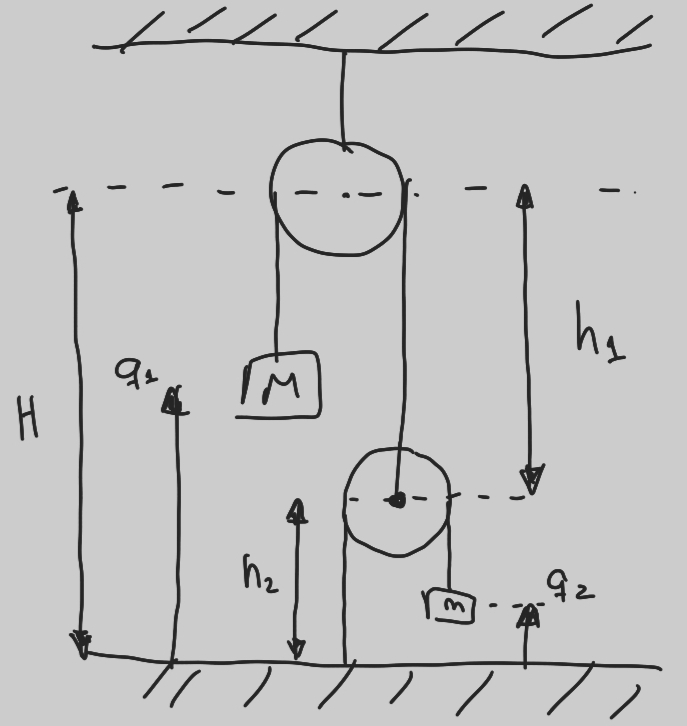
\includegraphics[width=0.5\textwidth]{hw1_p1.jpg}
\end{figure*}

\begin{solution}

Let $q_1,q_2,h_1,h_2$ be as described in the figure. $h_1+h_2=H$ is a constant.
Also, let $L_1,L_2$ be the length of the strings hung on the first and second
pulley. The following contraints follow
\begin{equation}
    L_1-h_1=H-q_1  
    \qquad\text{and}\qquad 2h_2-q_2=L_2
\end{equation}
We can combine these two constraints into
\begin{equation}
    q_2=4H-L_2-2L_1-2q_1=C-2q_1 
\end{equation}
where $C$ is a constant. Thus, the system only has one degree of freedom, where
$\dot{q_2}=-2\dot{q_1}$ and $\ddot{q_2}=-2\ddot{q_1}$. The Lagrange function is
thus
\begin{align}
    \LL&=\frac12M\dot{q_1}^2+\frac12m\dot{q_2}^2-Mgq_1-mgq_2\notag\\
       &=\frac12\qty(M+4m)\dot{q_1}^2-Mgq_1-mgC+2mgq_1
\end{align}
From Euler-Lagrange equation, we can write
\begin{equation}
    (M+4m)\ddot{q_1}=(2m-M)g
\end{equation}
The acceleration of the masses are then
\begin{subequations}
    \begin{align}
        \ddot{q_1}&=\frac{2m-M}{4m+M}g\\
        \ddot{q_2}&=-\frac{4m-2M}{4m+M}g
    \end{align} 
\end{subequations}


\end{solution}
    
\end{problem}

\begin{problem}{2}
A tunnel was dug between New York and Los Angeles such that a train which 
starts at rest in New York and moves along the tunnel by the gravitational pull 
only arrives in Los Angeles in the shortest possible time, neglecting air 
resistance and any other kind of friction. Following the discussion of the 
brachistochrone problem in Section 2.2 of Goldstein, calculate how far below 
the surface would the deepest point of the tunnel be if the distance between 
New York and Los Angeles is 4800\,\si{km} apart, while the radius of the Earth 
is approximately 6400\,\si{km}. Calculate also the time it would take for this 
train to travel between New York and Los Angeles. Mass of the Earth is 
$M\approx 6\times10^{24}$\,\si{kg}. 

\begin{solution}
    Assume the mass density, $\rho$, is uniform. Then at a radius $r\leq R$
    where $R$ is the Earth's radius, the enclosed mass within a volume $4\pi
    r^3/3$ is
    \begin{equation}
        M=M_E\frac{r^3}{R^3} 
    \end{equation}
    where $M_E$ is the total mass of the Earth. Now, the gravitational force on
    a train at $r$ with mass $m$ is
    \begin{equation}
        \vb{F}=-\frac{GMm}{r^2}\rhat=-\grad{V}
    \end{equation}
    So the gravitational potential is
    \begin{equation}
        V=-\int_0^r\vb{F}\vdot\rhat dr'
        =\frac{GM_E}{R^3}\int_0^rr'dr'
        =\frac{GM_Em}{2R^3}r^2=Cr^2
    \end{equation}
    where we have defined the constant $C\equiv GM_em/2R^3$. The total energy 
    is thus
    \begin{equation}
        E=\frac12mv^2+Cr^2    
    \end{equation}
    At departure on the surface ($r=R$), the train has zero speed, so
    $E_0=CR^2$. Then we can solve for the velocity
    \begin{equation}
        v=\sqrt{\frac{2C}{m}}\sqrt{R^2-r^2} 
    \end{equation}
    The train descends into the Earth to get from $A$ (New York) to $B$
    (Los Angeles). At some point $O$ ($r=r_0$), it reaches the deepest point   
    ($r=r_0$) into the Earth (see figure).
    \begin{figure*}[h]
        \centering
        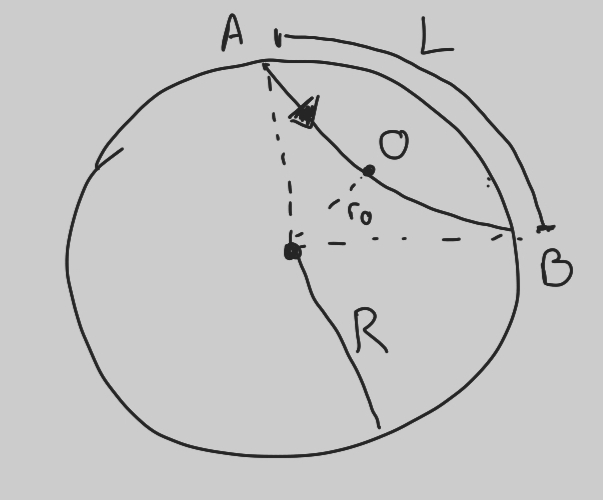
\includegraphics[width=0.5\textwidth]{hw1_p2.jpg}
    \end{figure*}
    Now, since the force is conservative, the time it 
    takes from $A$ to $O$ must be the same as that from $O$ to $B$. This time is
    \begin{equation}
        t_{O\to B}=\int_O^B\frac{ds}{v}
    \end{equation}
    The length element in polar coordinates is $ds^2=dr^2+r^2d\theta^2$. Setting
    $dr/d\theta=r'$, we can write
    \begin{equation}\label{p2:tOB}
        t_{O\to B}
        =\sqrt{\frac{m}{2C}}\int_{\theta_O}^{\theta_B}d\theta
        \frac{\sqrt{r^2+r'^2}}{v}
        =\sqrt{\frac{m}{2C}}\int_{\theta_O}^{\theta_B}d\theta
            \sqrt{\frac{r^2+r'^2}{R^2-r^2}}
    \end{equation}
    Let the integrand be
    \begin{equation}
        f(r,r')=\sqrt{\frac{r^2+r'^2}{R^2-r^2}}
        \Rightarrow\frac{\partial f}{\partial r'}=\frac1f\frac{r'}{R^2-r^2}
    \end{equation}
    The time $t_{O\to B}$ is minimized when
    \begin{equation}\label{p2:Et_1}
        \tilde{E}=f-r'\frac{\partial f}{\partial r'}
        =f\qty[1-\frac{r'^2}{f^2(R^2-r^2)}]
        =\frac{r^2}{\sqrt{(R^2-r^2)(r^2+r'^2)}}
    \end{equation}
    is constant. We can thus evaluate $\tilde{E}$ at $r=r_0$, where $r'=0$
    (because it is the lowest point)
    \begin{equation}\label{p2:Et_2}
        \eval{\tilde{E}}_{r=r_0}=\frac{r_0}{\sqrt{R^2-r_0^2}}
    \end{equation}
    From \eqref{p2:Et_1} and \eqref{p2:Et_2}, we can invert to find the
    differential equation
    \begin{equation}\label{p2:rprime}
        r'=\frac{dr}{d\theta}=\frac{Rr}{r_0}\sqrt{\frac{r^2-r_0^2}{R^2-r^2}} 
    \end{equation}
    Integrating, we get
    \begin{align}
        \int_{\theta_O}^{\theta_B}d\theta
        &=\frac{r_0}{R}\int_{r_0}^R\frac{dr}{r}\sqrt{\frac{R^2-r^2}{r^2-r_0^2}}
            \notag\\
        &=-\frac{r_0}{R}\frac{r_0-R}{r_0}\sin^{-1}
        \qty[\frac{\sqrt{(r_0^2-R^2)^2}}{r_0^2-R^2}]\tag{from Mathematica}\\
        &=-\frac{r_0-R}{R}\sin^{-1}(-1)\notag\\
        &=\frac\pi2\qty(\frac{r_0}{R}-1)
    \end{align}
    Note that $\theta_B<\theta_O$, so the RHS is also negative because $r_0<R$.
    By geometry, $\theta_O-\theta_B=\Delta\theta=L/2R$ where $L$ is the
    arc length from $A$ to $B$, so we can invert to find
    \begin{equation}
        r_0=R-\frac{L}{\pi}
        =6,400\,\si{km}-\frac{4,800\,\si{km}}{\pi}=4,872\,\si{km}
    \end{equation}
    Now that $r_0$ is known, we can plug \eqref{p2:rprime} into \eqref{p2:tOB}
    to get
    \begin{align}
        t_{O\to B}
        &=\sqrt{\frac{m}{2C}}\int_{r_0}^Rdr\frac{d\theta}{dr}
            \sqrt{\frac{r^2+r'^2}{R^2-r^2}}\notag\\
        &=\frac{\sqrt{R^2-r_0^2}}{R}\sqrt{\frac{m}{2C}}
            \int_{r_0}^R\frac{rdr}{\sqrt{(r^2-r_0^2)(R^2-r^2)}}
        &=\frac{\pi}{2}\sqrt{1-\qty(\frac{r_0}{R})^2}\sqrt{\frac{R^3}{GM_E}}
        &\approx824\,\si{s}
    \end{align}
    Then the total time it takes to get from $A$ to $B$ is $t_{A\to B}=2t_{O\to
    B}\approx27.5$\,\si{min}.
\end{solution}

\end{problem}


\end{document}
